\documentclass[plainboxedsections]{sciposter}
\usepackage{epsfig}
\usepackage{amsmath}
\usepackage{amssymb}
\usepackage{multicol}
\usepackage[brazil]{babel}
\usepackage{ucs}
\usepackage[utf8x]{inputenc}
\usepackage{color}

\title{Physimulation \\ Biblioteca Gráfica para Simulações de Física}
\author{Rafael Issao Miyagawa, Alberto Hideki Ueda\\ Orientador: José Coelho de Pina e João Pedro Kerr Catunda}
\institute{Instituto de Matemática e Estatística - Universidade de São Paulo}

\usepackage{lmodern}
\setmargins[1cm]
\definecolor{mainCol}{rgb}{1,1,1}
\definecolor{BoxCol}{rgb}{0.9,0.9,1}
\definecolor{TextCol}{rgb}{0.1,0.2,0.3}
\definecolor{SectionCol}{rgb}{0, 0, 0.4}
\newcommand{\blue}[1]{\textcolor{blue}{#1}}
\newcommand{\magenta}[1]{\textcolor{magenta}{#1}}
\begin{document}

\maketitle

\renewcommand{\papertype}{a2}
\renewcommand{\sectionsize}{\Huge}

\begin{multicols}{2}

  \section*{Motivação}
  \fontsize{50pt}{15pt}\selectfont
  \begin{itemize}
    \item Tornar interessante a disciplina de física
    \item Teorias da física aplicado na área de computação
    \item Simulações de diversos ambientes físicos
    \item Integração de exemplo com um Exercício Programa
  \end{itemize}

  \section*{Conceitos}
  \textbf{Passo de simulação} \\
  \\[1ex]
  Tempo utilizado para simular as interações entre objetos físicos. Pode ser fixo, variável ou semi-fixo
  \\[2ex]
  \textbf{Algoritmos Broad Phase} \\
  \\[1ex]
  Filtro para separar os objetos que devem passar pelo detecção de colisão
  \\[1ex]
  \underline{Sweep and Prune}\\
  \begin{figure}
    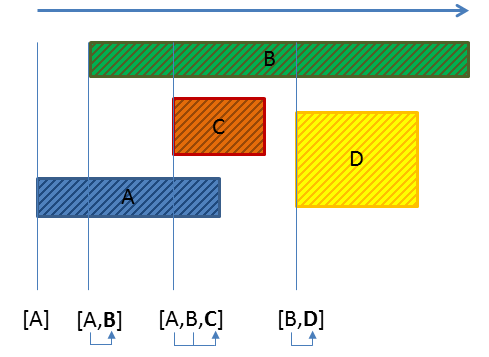
\includegraphics[scale=2]{sp.png}
  \end{figure}
  \underline{AABB Tree}\\
  \begin{figure}
    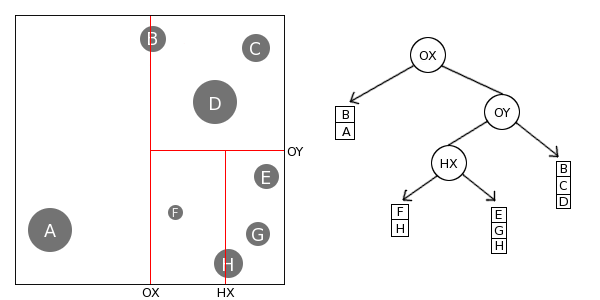
\includegraphics[scale=1.5]{aabb.png}
  \end{figure}
  \underline{Spatial Hashing}\\
  \begin{figure}
    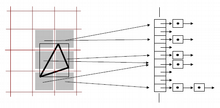
\includegraphics[scale=3]{sh.png}
  \end{figure}
  \\[1ex]
  \textbf{Detecção de Colisão} \\
  \\[1ex]
  \underline{Separating Axis Theorem}
  \\[1ex]
  Dizemos que existe uma colisão entre dois polígonos convexos s1 e s2 se e somente se não é possível desenhar uma linha que separe s1 e s2.
  \begin{figure}
    \centering
    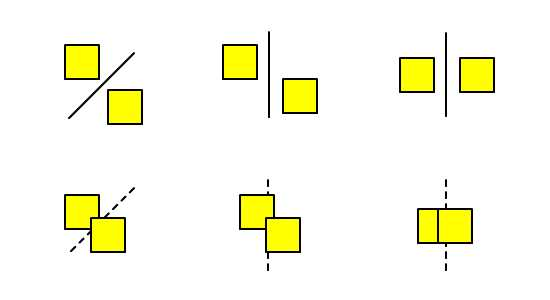
\includegraphics[scale=1.5]{SAT.jpg}
  \end{figure}

  \section*{Physimulation - Demonstração}
  \underline{Rocks}
  \\[1ex]
  \begin{figure}
      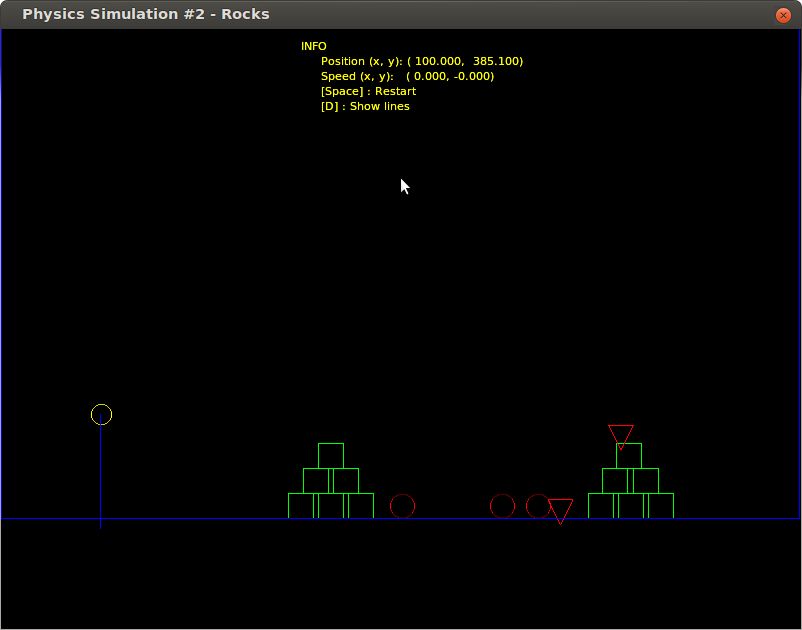
\includegraphics[scale=0.6]{esqueleto.png}
      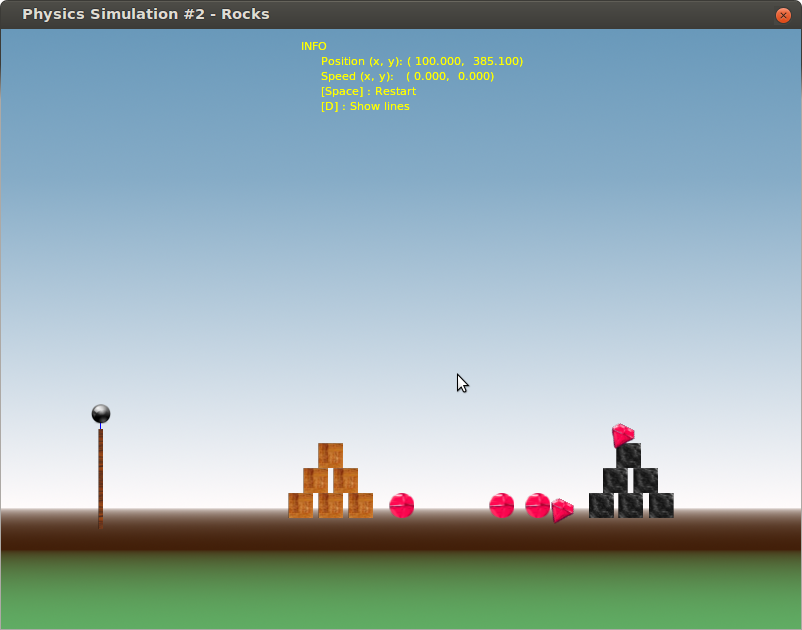
\includegraphics[scale=0.6]{comImagem.png}
  \end{figure}
  \\[1ex]
  \underline{Rocket landing}
  \\[1ex]
  \begin{figure}
    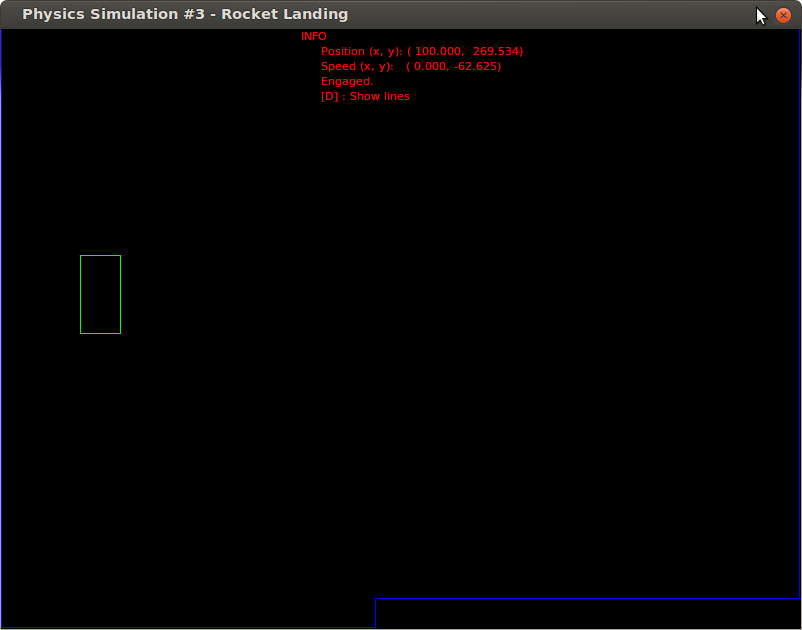
\includegraphics[scale=0.6]{lunarLandingE.png}
    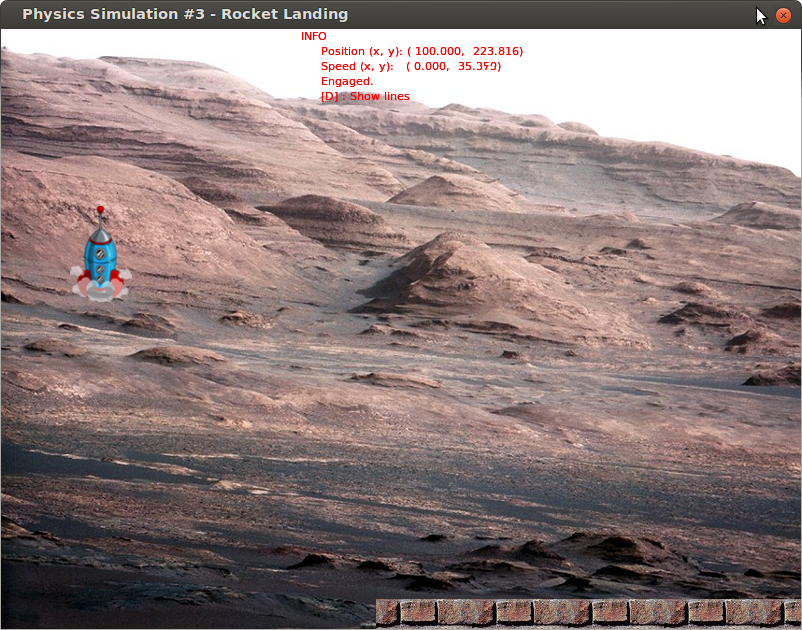
\includegraphics[scale=0.6]{lunarLanding.png}
  \end{figure}
  \\[1ex]
  \underline{Valley ball}
  \\[1ex]
  \begin{figure}
    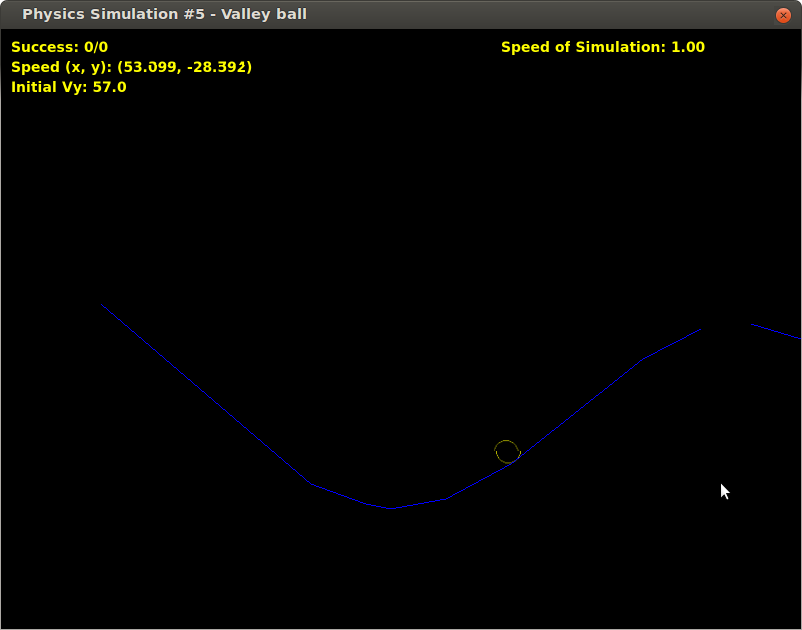
\includegraphics[scale=0.6]{valleyE.png}
    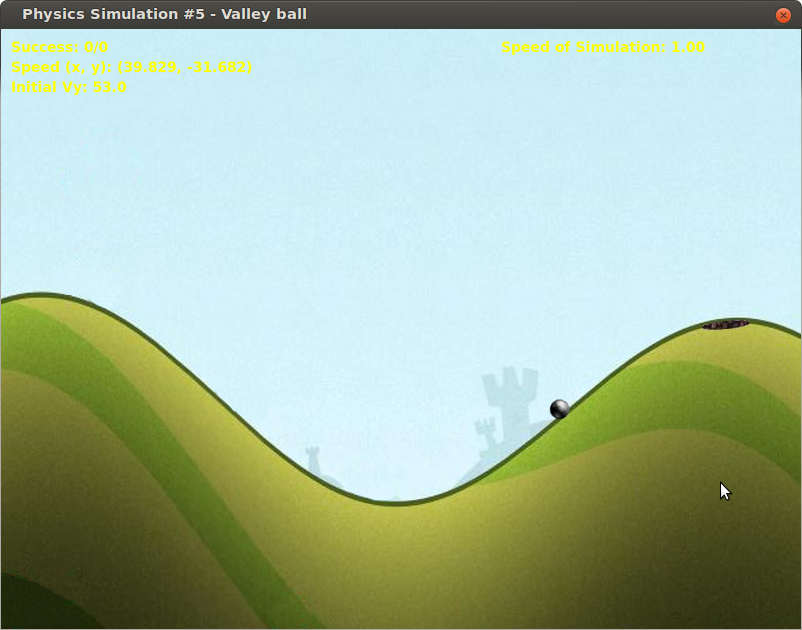
\includegraphics[scale=0.6]{valley.png}
  \end{figure}
\end{multicols}
\end{document}
